\documentclass[journal]{IEEEtran}

\usepackage{graphicx}

\begin{document}

\title{Reasoning in Artificial Neural Networks}

\author{
  \IEEEauthorblockN{Vasin Srisupavanich}
}

\maketitle

\begin{abstract}
Over the past decade, deep learning systems have enjoyed tremendous success in the area of computer vision and natural language understanding.
However, these systems still struggle in tasks which require deliberate thinking and reasoning process. 
Recently, many approaches to extend the capability of neural networks have emerged. 
This paper reviews several recent approaches which take inspiration from human's cognitive process and symbolic view of artificial intelligence
to solve reasoning tasks, and outlines future research directions in this challenging problem.
\end{abstract}

\begin{IEEEkeywords}
deep learning, artificial neural networks, reasoning, attention, memory, graph neural networks, neural-symbolic
\end{IEEEkeywords}

\section{Introduction}

\IEEEPARstart{T}{he} ability to reason is one of the most important features of human intelligence. 
It allows us to understand abstract concepts and make complex decisions.
Human excels at tasks that require deliberate thinking, such as planning and symbol manipulation, 
while the current state of machines are limited to simpler pattern matching problems.
Incorporating reasoning ability to machines has been a long standing goal, but a very difficult challenge in the field of Artificial Intelligence (AI). 
Solving this problem would mean a significant step toward artificial general intelligence, which will ultimately benefit humankind. 
This paper reviews recent approaches in building artificial neural networks (ANN) that can learn to reason, 
and overviews the current state of the art results and applications from deep learning systems with reasoning capability.

\section{Background}
According to \cite{bottou2014machine}, reasoning refers to the ability to ``algebraically manipulating previously acquired knowledge in order to answer a new question''.
Historically, the approach to create an AI system capable of reasoning has been from a symbolic point of view.
In a symbolic AI, knowledge is represented as symbols, and reasoning is the process of inference from knowledge and rules that are handcrafted by human.
However, this approach has been overshadowed by the success of deep learning in various domains in the past decades. 

Despite the astonishing power of the neural networks, they tend to learn statistical mapping between input and output, rather than the true causal relations. 
To address this shortcoming, ideas about symbols and reasoning in symbolic AI have been integrated in neural networks, 
either explicitly in a neural-symbolic approach, or implicitly in a graph neural networks model.
In addition, recent advances in deep learning, such as attention mechanism and the use of external memory, have been greatly inspired by the field of neuroscience, as 
human reasoning involves paying attention to specific parts of information and knowledge which are extracted from memory.

\section{Main Approaches}
\subsection{Attention Mechanism}
Attention mechanism was first introduced in 2014 in the context of machine translation \cite{bahdanau2014neural}, 
and became one of the most prominent tools in deep learning. 
This idea is loosely motivated by how human biological system works. 
In a human visual system, attention allows us to focus on specific region with high resolution, 
while ignoring other irrelevant information, making unfocused region blurry.
Similarly, in the context of machine translation, attention model enables the machine to focus on specific words at a time 
rather than the full sentence.

To illustrate, in a neural machine translation model (NMT), the architecture typically consists of an encoder-decoder (seq2seq) structure.
An encoder, usually a recurrent neural networks (RNN), learns to encode a source sentence into a fixed length vector.
Then the decoder network output the encoded vector into another language. Figure \ref{NMT}(a) shows the traditional encoder-decoder architecture.
The apparent problem of this architecture is that the model tends to forget relevant information in a long sentence.
With the addition of attention model (figure \ref{NMT}(b)), this problem is mitigated, 
as the decoder can learn to attend to different parts of the source sentence. 
The attention weights, which are from a feed forward neural networks, are jointly trained along with the encoder-decoder networks.

\begin{figure}[htb]
  \centering
  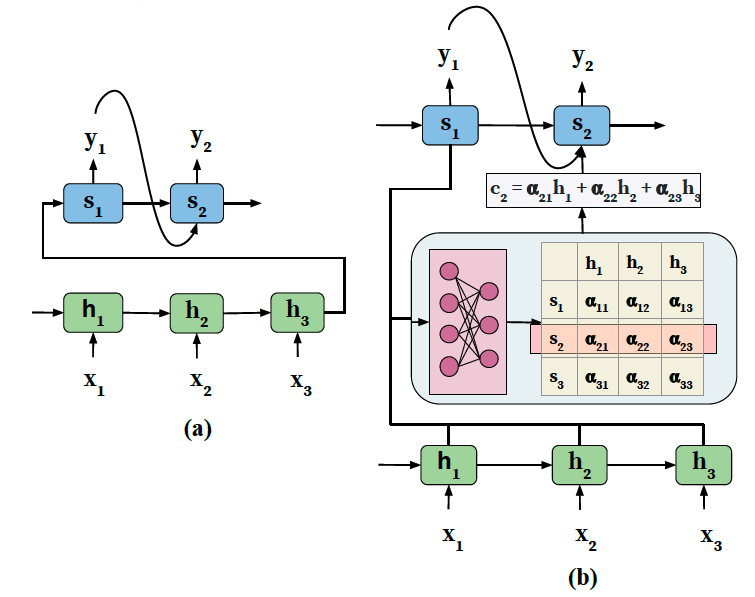
\includegraphics[width=0.7\columnwidth]{NMT.png}
  \caption{NMT architecture (a) traditional (b) with attention model.
  Figure from \cite{chaudhari1904attentive}}
  \label{NMT}
\end{figure}

In another influential paper by Xu et al \cite{xu2015show}, attention model is applied to generate caption from images. 
In this task, convolutional neural networks (CNN) is used as an encoder to extract features from raw images.
Then a long short-term memory network (LSTM) is used to generate the words, conditioned on the attention weights.
Figure \ref{attention} demonstrates how the model learns to attend to specific part of the image with the corresponding word. 
Also proposed in \cite{xu2015show}, the attention model can be classified in two types: soft and hard attention. 
In soft attention, the model is smooth and differentiable end-to-end, and the context vector is computed by the weighted average of the whole image. 
In contrast, in hard attention, the context vector is computed from stochastically sampled patch of image, 
which makes the model non-differentiable and requires reinforcement learning to train.

\begin{figure}[htb]
  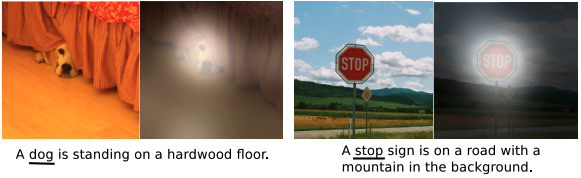
\includegraphics[width=\linewidth]{attention.png}
  \caption{Visualization of the attended region conditioned on the corresponding word.
  Figure from \cite{xu2015show}}
  \label{attention}
\end{figure}

\subsection{Memory Augmented Neural Networks}
Similar to human, in order to retrieve the information necessary for the desired tasks, a machine needs to maintain some memory that needs to be efficiently organized and queried. 
This is particularly essential for complex tasks, such as multi-hop reasoning. Traditional RNN and its variant LSTM can memorize information in the hidden states,
however, they are limited to only short term dependencies. Recent approaches to alleviate this issues involve explicit memory representation and the use of external memory, 
as proposed in Neural Turing Machine \cite{graves2014neural} and Memory Networks \cite{weston2014memory}. 

A Neural Turing Machine (NTM) contains two major components: a neural network controller and a memory bank (Figure \ref{NTM}). 
A controller can be any type of neural networks, such as feed forward or RNN, and is responsible for read and write operations on the memory matrix.
The read and write operations are done selectively by soft attention mechanism, making every components fully differentiable, 
and thereby the whole model can be trained using gradient descent. The experiments reported in \cite{graves2014neural} have shown that NTM significantly
outperforms traditional LSTM in tasks, such as copying and sorting.

\begin{figure}[htb]
  \centering
  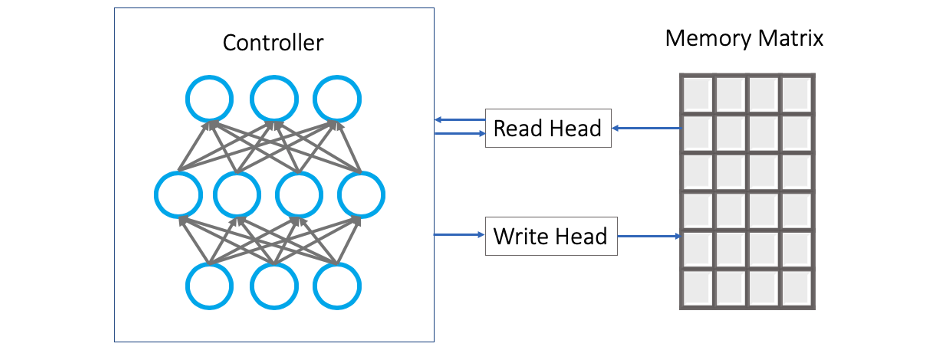
\includegraphics[width=0.8\columnwidth]{NTM.png}
  \caption{Architecture of Neural Turing Machine}
  \label{NTM}
\end{figure}

Another recent neural networks model, utilizing both attention and memory, designed to facilitate explicit reasoning is the MAC networks \cite{hudson2018compositional}.
In contrast to NTM, the MAC model doesn't utilize a global external memory. Instead, each node (MAC cell) is recurrent, and has its own memory and control state.
In contrast to the traditional neural networks, the separation between control and memory encourages the networks to 
learn the computational process and reasoning operations, rather than to approximate direct transformation between the input and output.
Figure \ref{mac-clevr} shows the result of the MAC networks from a visual reasoning task using CLEVR data set \cite{johnson2017clevr}. 
The MAC networks was able to achieve 98.94\% accuracy, halving the error rate from the best prior model.
\begin{figure}[htb]
  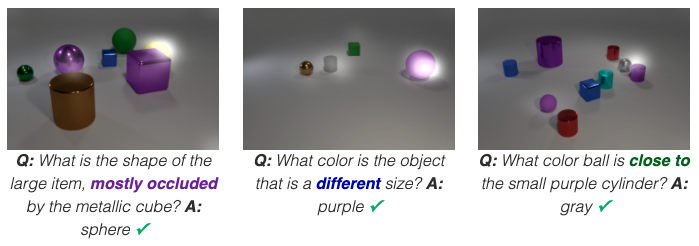
\includegraphics[width=\linewidth]{mac-clevr.png}
  \caption{Example of MAC networks performing novel visual reasoning task. Figure from \cite{hudson2018compositional}}
  \label{mac-clevr}
\end{figure}

\subsection{Neural-Symbolic}
The aim of the neural-symbolic approach is to combine symbolic AI's ability to reason 
and neural networks' ability to learn to improve over time. 
The complementary strengths of this hybrid AI system has given impressive results in many applications, 
and is gaining more traction recently in the AI community.

In a visual question answering (VQA) task, a recent neural-symbolic system, NS-CL \cite{Mao2019NeuroSymbolic} employed deep representation learning (CNN, LSTM)
for visual recognition and language understanding, while the reasoning part is solved by symbolic program execution.
The framework proposed in NS-CL contains three separate modules: 
a \textit{visual module} where the objects are detected and vector representations are extracted, 
a \textit{semantic parser} where the question text is parsed into a tree of pre-defined domain specific language (DSL) of executable program,
and a \textit{symbolic program} executer which takes in the parsed program and vector representation of objects to derive the answer. 

\begin{figure}[htb]
  \centering
  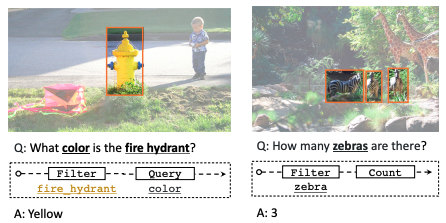
\includegraphics[width=0.8\columnwidth]{nscl.png}
  \caption{Result of NS-CL on the VQS dataset. Figure from \cite{Mao2019NeuroSymbolic}}
  \label{nscl}
\end{figure}

The experiments reported in \cite{Mao2019NeuroSymbolic} shows that this method requires significantly less amount of training data to accurately answer questions, 
and is able to generalize to new scenes and questions better than other methods. 
Moreover, its results are fully interpretable, as the execution trace is visible, 
unlike a black box system in a traditional ANN.
Figure \ref{nscl} shows the result of this model on the VQS dataset, along with the generated symbolic programs. 
However, one significant limitation is that the symbolic functions (DSL) need to be pre-defined. 
As shown in figure \ref{nscl}, functions such as filter, count and query are hard-coded into the system, 
which make it difficult to translate into the real-world system.

\subsection{Graph Neural Networks}

Graph neural networks (GNN) can be described as a type of neural networks which operates on the graph structure.
It is particularly suited for tasks where data are represented as graph with complex relationship and interdependency between objects.
A graph is a data structure consisted of vertices (nodes) and edges.
The edge can either be directed or undirected depending on the relationship between objects.
In GNN, the node, edge and output can be flexibly represented in different types depending on the task. 
For instance, the node can represent the patch of the image or a sequence of words when the input is text.

It is reported that GNN is well suited for relational reasoning tasks, because of the strong relational inductive bias \cite{graphnetworks}.
In contrast to CNN, where the inductive bias is the locality of the receptive field, 
and RNN where the bias is the sequentiality of data, GNN can express arbitrary relationship among entities. 
Another recent paper \cite{xu2019can} studied what tasks a neural network can learn to reason. 
The result revealed that the performance of the neural networks increases
when the computational structure of the neural networks aligns with the algorithmic structure of the reasoning process. 
Moreover, GNN is able to generalize better than other types of neural networks, 
as its underlying reasoning process resembles dynamic programming.

To illustrate the use of the graph networks, a recent model called Neural State Machine (NSM) \cite{hudson2019learning} utilized graph structure to represent the scene of an image in a VQA task.
This model works in two stages: modeling and inference. 
In the modeling stage, the image is decomposed into a probabilistic graph that captures the semantic of the visual scene.
The node corresponds to object within the image, while the edge represents both spatial and semantic relations.
In the inference stage, the sequential reasoning process is performed over the graph by iteratively traversing its node guided by the question.
Figure \ref{nsm} shows the overall process of NSM, with the generated scene graph.
As reported in \cite{hudson2019learning}, this model has achieved state-of-the-art result in various visual reasoning benchmarks.

\begin{figure}[htb]
  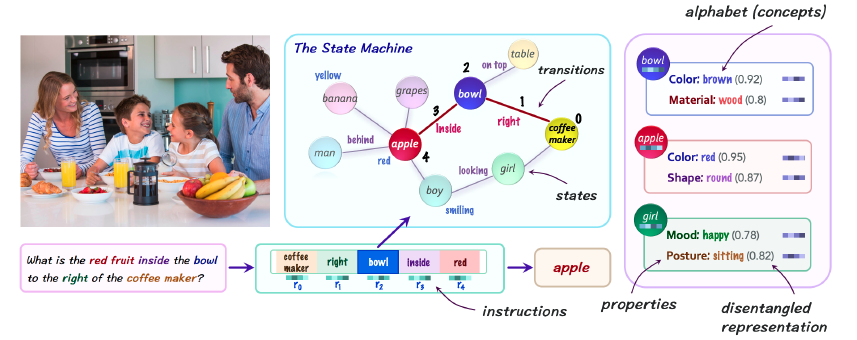
\includegraphics[width=\linewidth]{NSM.png}
  \caption{Overall process of Neural State Machine. Figure from \cite{hudson2019learning}}
  \label{nsm}
\end{figure}

\section{Discussion}

We have seen several approaches in building a neural networks with reasoning capability.
The attention mechanism allows the model to focus on the specific part of information, 
but this method alone cannot be used to solve the reasoning task.
Similar to a working memory in the human brain, 
adding explicit external memory gives the model the ability to utilize previous knowledge.
However, the networks with global memory can be extremely difficult to train. 
In a neural-symbolic system, the results can be more interpretable and explainable,
still, this come with a cost of fixed symbolic functions, making it difficult to scale into practice.
In contrast to neural-symbolic approach, a GNN can be used to recreate the symbolic structure, 
while maintaining the end-to-end differentiability. Yet, many problems and processes cannot be easily represented as graph.

Although these approaches have shown promising results in various reasoning benchmarks, 
there are still a lot of open questions in how to alleviate each of the weakness. 
To augment neural networks with memory, questions of how information are stored 
and which type of memory to use, are still need to be solved. 
Moreover, in order to generalize reasoning operations to unseen tasks, 
we would need to find better ways to represent data, or concepts in a disentangle way.
However, considering the recent breakthrough and the similarity with human's cognitive process, 
the use of attention mechanism, memory, and the right inductive prior, could be the right step towards making a machine that is more intelligent.

\bibliographystyle{IEEEtran}
\bibliography{references}

\end{document}